%\newpage
\section{Widerstands Messung}
Jeder Widerstand wird mit vier verschiedenen Me"smethoden in einer Stromrichtung vermessen.
Der gleiche Widerstand wird auch mit den gleichen vier Me"smethoden in die andere Stromrichtung vermessen.
Die Messung in die Gegenrichtung wird nur f\"ur die Erkennung auf Widerstand benutzt.
Wenn die Abweichung dieser beiden Messungen zu gro"s ist, ist es kein Widerstand.

\subsection{Widerstandsmessung mit den 680 Ohm Widerst\"anden}
Die Messung des unbekannten Widerstandes Rx wird in zwei verschiedenen Wegen mit den \(680\Omega\) Pr\"azisionswiderst\"anden
 durchgef\"uhrt.
Das Schaltbild dieser Messungen mit Testpin 1 (TP1) und Testpin 3 (TP3) werden vereinfacht in Abbildung~\ref{fig:RL1mes} und Abbildung~\ref{fig:RL2mes} als ein Beispiel von den sechs Kombinationsm\"oglichkeiten gezeigt.

\begin{figure}[H]
\centering

\includegraphics[]{../FIG/ResistormessL1.eps}
\caption{Messung Type 1 mit \(680\Omega\) }
\label{fig:RL1mes}
\end{figure}

\begin{figure}[H]
 \centering
 
\includegraphics[]{../FIG/ResistormessL2.eps}
 \caption{Messung Type 2 mit \(680\Omega\) }
\label{fig:RL2mes}
\end{figure}

Auf der linken Seite wird der Testpin 1 und auf der rechten Seite der Testpin 3 gezeigt.
In beiden Schaltungen kann man erkennen, da"s der Anschlu"s 3 (TP3) mit VCC und die linke Seite (TP1) mit
GND verbunden ist.
Die Stromrichtung durch den Widerstand Rx ist immer die gleiche.
Die Werte f\"ur auf Ausgang geschaltete Ports werden mit roter Farbe dargestellt, 
die Werte f\"ur die Eing\"ange werden mit blauer Farbe dargestellt, inaktive Ports sind schwarz.
In beiden gezeigten Me"smethoden sollte der Strom den gleichen Wert haben, weil die Summe der Widerst\"ande zwischen
VCC und GND gleich ist, vorausgesetzt die eingebauten Widerst\"ande sind gleich.
Normalerweise sind die gemessenen Spannungen aber nicht gleich, weil die Reihenfolge
der Widerst\"ande vertauscht ist.

Das V Symbol innerhalb eines Kreises markiert die Ports, die f\"ur die Spannungsmessung benutzt werden.
In beiden Konfigurationen kann der Wert des Widerstandes Rx aus den bekannten Widerstandswerten
und den gemessenen Spannungen berechnet werden, wenn das Verh\"altnis des Widerstands Rx und den \(680\Omega\) Widerst\"anden
 nicht zu hoch ist.
Der theoretische Spannungsverlauf wird in Abbildung~\ref{fig:RLvtot} gezeigt, wobei die Widerstandswerte 
in logarithmischer Skalierung dargestellt sind.
\begin{figure}[H]
\centering
% GNUPLOT: LaTeX picture with Postscript
\begingroup
  \makeatletter
  \providecommand\color[2][]{%
    \GenericError{(gnuplot) \space\space\space\@spaces}{%
      Package color not loaded in conjunction with
      terminal option `colourtext'%
    }{See the gnuplot documentation for explanation.%
    }{Either use 'blacktext' in gnuplot or load the package
      color.sty in LaTeX.}%
    \renewcommand\color[2][]{}%
  }%
  \providecommand\includegraphics[2][]{%
    \GenericError{(gnuplot) \space\space\space\@spaces}{%
      Package graphicx or graphics not loaded%
    }{See the gnuplot documentation for explanation.%
    }{The gnuplot epslatex terminal needs graphicx.sty or graphics.sty.}%
    \renewcommand\includegraphics[2][]{}%
  }%
  \providecommand\rotatebox[2]{#2}%
  \@ifundefined{ifGPcolor}{%
    \newif\ifGPcolor
    \GPcolortrue
  }{}%
  \@ifundefined{ifGPblacktext}{%
    \newif\ifGPblacktext
    \GPblacktexttrue
  }{}%
  % define a \g@addto@macro without @ in the name:
  \let\gplgaddtomacro\g@addto@macro
  % define empty templates for all commands taking text:
  \gdef\gplbacktext{}%
  \gdef\gplfronttext{}%
  \makeatother
  \ifGPblacktext
    % no textcolor at all
    \def\colorrgb#1{}%
    \def\colorgray#1{}%
  \else
    % gray or color?
    \ifGPcolor
      \def\colorrgb#1{\color[rgb]{#1}}%
      \def\colorgray#1{\color[gray]{#1}}%
      \expandafter\def\csname LTw\endcsname{\color{white}}%
      \expandafter\def\csname LTb\endcsname{\color{black}}%
      \expandafter\def\csname LTa\endcsname{\color{black}}%
      \expandafter\def\csname LT0\endcsname{\color[rgb]{1,0,0}}%
      \expandafter\def\csname LT1\endcsname{\color[rgb]{0,1,0}}%
      \expandafter\def\csname LT2\endcsname{\color[rgb]{0,0,1}}%
      \expandafter\def\csname LT3\endcsname{\color[rgb]{1,0,1}}%
      \expandafter\def\csname LT4\endcsname{\color[rgb]{0,1,1}}%
      \expandafter\def\csname LT5\endcsname{\color[rgb]{1,1,0}}%
      \expandafter\def\csname LT6\endcsname{\color[rgb]{0,0,0}}%
      \expandafter\def\csname LT7\endcsname{\color[rgb]{1,0.3,0}}%
      \expandafter\def\csname LT8\endcsname{\color[rgb]{0.5,0.5,0.5}}%
    \else
      % gray
      \def\colorrgb#1{\color{black}}%
      \def\colorgray#1{\color[gray]{#1}}%
      \expandafter\def\csname LTw\endcsname{\color{white}}%
      \expandafter\def\csname LTb\endcsname{\color{black}}%
      \expandafter\def\csname LTa\endcsname{\color{black}}%
      \expandafter\def\csname LT0\endcsname{\color{black}}%
      \expandafter\def\csname LT1\endcsname{\color{black}}%
      \expandafter\def\csname LT2\endcsname{\color{black}}%
      \expandafter\def\csname LT3\endcsname{\color{black}}%
      \expandafter\def\csname LT4\endcsname{\color{black}}%
      \expandafter\def\csname LT5\endcsname{\color{black}}%
      \expandafter\def\csname LT6\endcsname{\color{black}}%
      \expandafter\def\csname LT7\endcsname{\color{black}}%
      \expandafter\def\csname LT8\endcsname{\color{black}}%
    \fi
  \fi
  \setlength{\unitlength}{0.0500bp}%
  \begin{picture}(7200.00,5040.00)%
    \gplgaddtomacro\gplbacktext{%
      \csname LTb\endcsname%
      \put(1078,704){\makebox(0,0)[r]{\strut{} 0}}%
      \csname LTb\endcsname%
      \put(1078,1518){\makebox(0,0)[r]{\strut{} 1000}}%
      \csname LTb\endcsname%
      \put(1078,2332){\makebox(0,0)[r]{\strut{} 2000}}%
      \csname LTb\endcsname%
      \put(1078,3147){\makebox(0,0)[r]{\strut{} 3000}}%
      \csname LTb\endcsname%
      \put(1078,3961){\makebox(0,0)[r]{\strut{} 4000}}%
      \csname LTb\endcsname%
      \put(1078,4775){\makebox(0,0)[r]{\strut{} 5000}}%
      \csname LTb\endcsname%
      \put(1210,484){\makebox(0,0){\strut{}100m}}%
      \csname LTb\endcsname%
      \put(2142,484){\makebox(0,0){\strut{}1 }}%
      \csname LTb\endcsname%
      \put(3074,484){\makebox(0,0){\strut{}10 }}%
      \csname LTb\endcsname%
      \put(4007,484){\makebox(0,0){\strut{}100 }}%
      \csname LTb\endcsname%
      \put(4939,484){\makebox(0,0){\strut{}1k}}%
      \csname LTb\endcsname%
      \put(5871,484){\makebox(0,0){\strut{}10k}}%
      \csname LTb\endcsname%
      \put(6803,484){\makebox(0,0){\strut{}100k}}%
      \put(176,2739){\rotatebox{-270}{\makebox(0,0){\strut{}voltage / mV}}}%
      \put(4006,154){\makebox(0,0){\strut{}resistor Rx / Ohm}}%
      \put(4006,4665){\makebox(0,0){\strut{}}}%
      \put(286,110){\makebox(0,0)[l]{\strut{}}}%
    }%
    \gplgaddtomacro\gplfronttext{%
      \csname LTb\endcsname%
      \put(3594,3094){\makebox(0,0)[r]{\strut{}PC2, type 1}}%
      \csname LTb\endcsname%
      \put(3594,2874){\makebox(0,0)[r]{\strut{}PC0, type 2}}%
    }%
    \gplbacktext
    \put(0,0){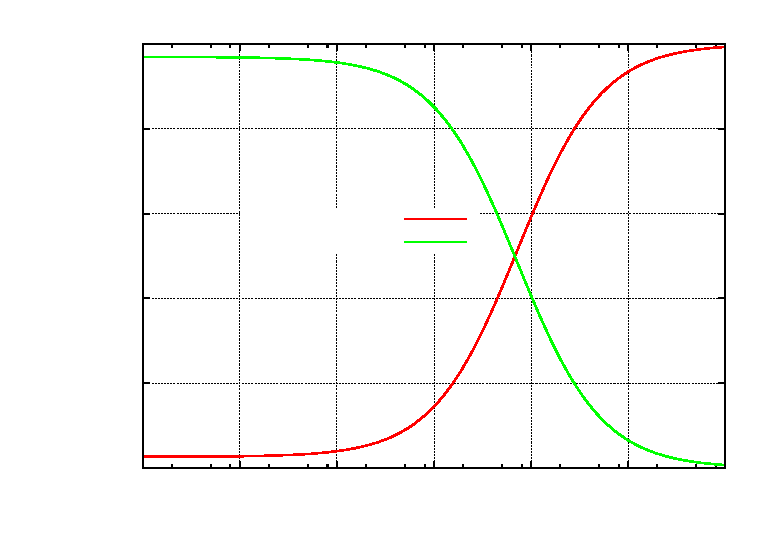
\includegraphics{../GNU/RLvtot}}%
    \gplfronttext
  \end{picture}%
\endgroup

\caption{Spannung von Type 1 und Type 2 Messungen mit \(680\Omega\) }
\label{fig:RLvtot}
\end{figure}
Die Verlauf f\"ur Messung Type 1 wird in Abbildung~\ref{fig:RLvlow} mit gespreizter Darstellung f\"ur die unteren Widerstandwerte gezeigt.
Wie man sehen kann, braucht man eine bessere ADC Aufl\"osung als die Standard 4,9mV bei der 5V ADC Referenz, um richtige
Widerstandswerte von der gemessenen Spannung unter \(2\Omega\) zu erhalten.
Es gibt nur drei ADC Stufen mit der 5V Referenz zwischen \(0\Omega\) und \(2\Omega\).
Hier kann die Bereichsumschaltung mit der AUTOSCALE\_ADC Option helfen.
Der gleiche gespreizte Bereich f\"ur die Type 2 Messung wird in Abbildung~\ref{fig:RLvhigh} gezeigt.
Ungl\"ucklicherweise kann man nicht die h\"ohere ADC Aufl\"osung f\"ur Me"smethode Type 2 benutzen,
weil die Spannung zu hoch ist und unser ATmega keine differenziellen ADC Eing\"ange besitzt.
Die Messungen mit den \(680\Omega\) Widerst\"anden werden bis zu einem Widerstandswert von 
\(28k\Omega\) (Spannung ist unter 120mV) zur Bestimmung des Me"sergebnisses verwendet.

F\"ur h\"ohere Widerstandswerte werden Messungen mit den \(470k\Omega\) Widerst\"anden benutzt.
Der Mittelwert von beiden Messungen wird f\"ur den angezeigten Widerstandwert benutzt, wenn alle Messungen ergeben,
da"s es kein anderes Bauteil ist.
Wenn die AUTOSCALE\_ADC Funktion benutzt wird und eine der gemessenen Spannungen f\"ur beide Versionen unter 0,98V liegt,
wird ein gewichteter Mittelwert mit Faktor vier f\"ur die Messung mit der Spannung unter 0,98V benutzt. Der andere Wert wird mit Faktor eins bewertet.
Das wird wegen der Faktor vier besseren Aufl\"osung dieser Messung gemacht.
Faktor vier wird nur f\"ur ATmega88, ATmega168 und ATmega328 Prozessoren verwendet, f\"ur ATmega8 wird ein
Faktor zwei als Wichtung benutzt wenn die Spannung unter 0,98V ist, weil die ADC Referenzspannung hier 2,54V statt 1,1V betr"agt.

\begin{figure}[H]
  \begin{subfigure}[b]{9cm}
    \centering
    \resizebox{9cm}{!}{% GNUPLOT: LaTeX picture with Postscript
\begingroup
  \makeatletter
  \providecommand\color[2][]{%
    \GenericError{(gnuplot) \space\space\space\@spaces}{%
      Package color not loaded in conjunction with
      terminal option `colourtext'%
    }{See the gnuplot documentation for explanation.%
    }{Either use 'blacktext' in gnuplot or load the package
      color.sty in LaTeX.}%
    \renewcommand\color[2][]{}%
  }%
  \providecommand\includegraphics[2][]{%
    \GenericError{(gnuplot) \space\space\space\@spaces}{%
      Package graphicx or graphics not loaded%
    }{See the gnuplot documentation for explanation.%
    }{The gnuplot epslatex terminal needs graphicx.sty or graphics.sty.}%
    \renewcommand\includegraphics[2][]{}%
  }%
  \providecommand\rotatebox[2]{#2}%
  \@ifundefined{ifGPcolor}{%
    \newif\ifGPcolor
    \GPcolortrue
  }{}%
  \@ifundefined{ifGPblacktext}{%
    \newif\ifGPblacktext
    \GPblacktexttrue
  }{}%
  % define a \g@addto@macro without @ in the name:
  \let\gplgaddtomacro\g@addto@macro
  % define empty templates for all commands taking text:
  \gdef\gplbacktext{}%
  \gdef\gplfronttext{}%
  \makeatother
  \ifGPblacktext
    % no textcolor at all
    \def\colorrgb#1{}%
    \def\colorgray#1{}%
  \else
    % gray or color?
    \ifGPcolor
      \def\colorrgb#1{\color[rgb]{#1}}%
      \def\colorgray#1{\color[gray]{#1}}%
      \expandafter\def\csname LTw\endcsname{\color{white}}%
      \expandafter\def\csname LTb\endcsname{\color{black}}%
      \expandafter\def\csname LTa\endcsname{\color{black}}%
      \expandafter\def\csname LT0\endcsname{\color[rgb]{1,0,0}}%
      \expandafter\def\csname LT1\endcsname{\color[rgb]{0,1,0}}%
      \expandafter\def\csname LT2\endcsname{\color[rgb]{0,0,1}}%
      \expandafter\def\csname LT3\endcsname{\color[rgb]{1,0,1}}%
      \expandafter\def\csname LT4\endcsname{\color[rgb]{0,1,1}}%
      \expandafter\def\csname LT5\endcsname{\color[rgb]{1,1,0}}%
      \expandafter\def\csname LT6\endcsname{\color[rgb]{0,0,0}}%
      \expandafter\def\csname LT7\endcsname{\color[rgb]{1,0.3,0}}%
      \expandafter\def\csname LT8\endcsname{\color[rgb]{0.5,0.5,0.5}}%
    \else
      % gray
      \def\colorrgb#1{\color{black}}%
      \def\colorgray#1{\color[gray]{#1}}%
      \expandafter\def\csname LTw\endcsname{\color{white}}%
      \expandafter\def\csname LTb\endcsname{\color{black}}%
      \expandafter\def\csname LTa\endcsname{\color{black}}%
      \expandafter\def\csname LT0\endcsname{\color{black}}%
      \expandafter\def\csname LT1\endcsname{\color{black}}%
      \expandafter\def\csname LT2\endcsname{\color{black}}%
      \expandafter\def\csname LT3\endcsname{\color{black}}%
      \expandafter\def\csname LT4\endcsname{\color{black}}%
      \expandafter\def\csname LT5\endcsname{\color{black}}%
      \expandafter\def\csname LT6\endcsname{\color{black}}%
      \expandafter\def\csname LT7\endcsname{\color{black}}%
      \expandafter\def\csname LT8\endcsname{\color{black}}%
    \fi
  \fi
  \setlength{\unitlength}{0.0500bp}%
  \begin{picture}(7200.00,5040.00)%
    \gplgaddtomacro\gplbacktext{%
      \csname LTb\endcsname%
      \put(946,704){\makebox(0,0)[r]{\strut{} 130}}%
      \csname LTb\endcsname%
      \put(946,995){\makebox(0,0)[r]{\strut{} 135}}%
      \csname LTb\endcsname%
      \put(946,1286){\makebox(0,0)[r]{\strut{} 140}}%
      \csname LTb\endcsname%
      \put(946,1576){\makebox(0,0)[r]{\strut{} 145}}%
      \csname LTb\endcsname%
      \put(946,1867){\makebox(0,0)[r]{\strut{} 150}}%
      \csname LTb\endcsname%
      \put(946,2158){\makebox(0,0)[r]{\strut{} 155}}%
      \csname LTb\endcsname%
      \put(946,2449){\makebox(0,0)[r]{\strut{} 160}}%
      \csname LTb\endcsname%
      \put(946,2740){\makebox(0,0)[r]{\strut{} 165}}%
      \csname LTb\endcsname%
      \put(946,3030){\makebox(0,0)[r]{\strut{} 170}}%
      \csname LTb\endcsname%
      \put(946,3321){\makebox(0,0)[r]{\strut{} 175}}%
      \csname LTb\endcsname%
      \put(946,3612){\makebox(0,0)[r]{\strut{} 180}}%
      \csname LTb\endcsname%
      \put(946,3903){\makebox(0,0)[r]{\strut{} 185}}%
      \csname LTb\endcsname%
      \put(946,4193){\makebox(0,0)[r]{\strut{} 190}}%
      \csname LTb\endcsname%
      \put(946,4484){\makebox(0,0)[r]{\strut{} 195}}%
      \csname LTb\endcsname%
      \put(946,4775){\makebox(0,0)[r]{\strut{} 200}}%
      \csname LTb\endcsname%
      \put(1078,484){\makebox(0,0){\strut{} 0}}%
      \csname LTb\endcsname%
      \put(1651,484){\makebox(0,0){\strut{} 1}}%
      \csname LTb\endcsname%
      \put(2223,484){\makebox(0,0){\strut{} 2}}%
      \csname LTb\endcsname%
      \put(2796,484){\makebox(0,0){\strut{} 3}}%
      \csname LTb\endcsname%
      \put(3368,484){\makebox(0,0){\strut{} 4}}%
      \csname LTb\endcsname%
      \put(3941,484){\makebox(0,0){\strut{} 5}}%
      \csname LTb\endcsname%
      \put(4513,484){\makebox(0,0){\strut{} 6}}%
      \csname LTb\endcsname%
      \put(5086,484){\makebox(0,0){\strut{} 7}}%
      \csname LTb\endcsname%
      \put(5658,484){\makebox(0,0){\strut{} 8}}%
      \csname LTb\endcsname%
      \put(6231,484){\makebox(0,0){\strut{} 9}}%
      \csname LTb\endcsname%
      \put(6803,484){\makebox(0,0){\strut{} 10}}%
      \put(176,2739){\rotatebox{-270}{\makebox(0,0){\strut{}voltage / mV}}}%
      \put(3940,154){\makebox(0,0){\strut{}resistor Rx / Ohm}}%
      \put(3940,4665){\makebox(0,0){\strut{}}}%
    }%
    \gplgaddtomacro\gplfronttext{%
      \csname LTb\endcsname%
      \put(5816,4602){\makebox(0,0)[r]{\strut{}PC2, type 1}}%
    }%
    \gplbacktext
    \put(0,0){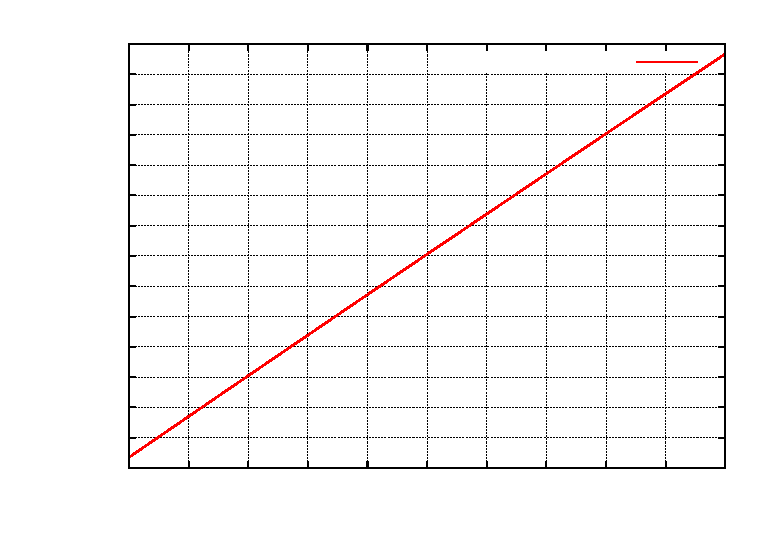
\includegraphics{../GNU/RLvlow}}%
    \gplfronttext
  \end{picture}%
\endgroup
}
    \caption{Type 1 Messung}
    \label{fig:RLvlow}
  \end{subfigure}
  ~
  \begin{subfigure}[b]{9cm}
    \centering
    \resizebox{9cm}{!}{% GNUPLOT: LaTeX picture with Postscript
\begingroup
  \makeatletter
  \providecommand\color[2][]{%
    \GenericError{(gnuplot) \space\space\space\@spaces}{%
      Package color not loaded in conjunction with
      terminal option `colourtext'%
    }{See the gnuplot documentation for explanation.%
    }{Either use 'blacktext' in gnuplot or load the package
      color.sty in LaTeX.}%
    \renewcommand\color[2][]{}%
  }%
  \providecommand\includegraphics[2][]{%
    \GenericError{(gnuplot) \space\space\space\@spaces}{%
      Package graphicx or graphics not loaded%
    }{See the gnuplot documentation for explanation.%
    }{The gnuplot epslatex terminal needs graphicx.sty or graphics.sty.}%
    \renewcommand\includegraphics[2][]{}%
  }%
  \providecommand\rotatebox[2]{#2}%
  \@ifundefined{ifGPcolor}{%
    \newif\ifGPcolor
    \GPcolortrue
  }{}%
  \@ifundefined{ifGPblacktext}{%
    \newif\ifGPblacktext
    \GPblacktexttrue
  }{}%
  % define a \g@addto@macro without @ in the name:
  \let\gplgaddtomacro\g@addto@macro
  % define empty templates for all commands taking text:
  \gdef\gplbacktext{}%
  \gdef\gplfronttext{}%
  \makeatother
  \ifGPblacktext
    % no textcolor at all
    \def\colorrgb#1{}%
    \def\colorgray#1{}%
  \else
    % gray or color?
    \ifGPcolor
      \def\colorrgb#1{\color[rgb]{#1}}%
      \def\colorgray#1{\color[gray]{#1}}%
      \expandafter\def\csname LTw\endcsname{\color{white}}%
      \expandafter\def\csname LTb\endcsname{\color{black}}%
      \expandafter\def\csname LTa\endcsname{\color{black}}%
      \expandafter\def\csname LT0\endcsname{\color[rgb]{1,0,0}}%
      \expandafter\def\csname LT1\endcsname{\color[rgb]{0,1,0}}%
      \expandafter\def\csname LT2\endcsname{\color[rgb]{0,0,1}}%
      \expandafter\def\csname LT3\endcsname{\color[rgb]{1,0,1}}%
      \expandafter\def\csname LT4\endcsname{\color[rgb]{0,1,1}}%
      \expandafter\def\csname LT5\endcsname{\color[rgb]{1,1,0}}%
      \expandafter\def\csname LT6\endcsname{\color[rgb]{0,0,0}}%
      \expandafter\def\csname LT7\endcsname{\color[rgb]{1,0.3,0}}%
      \expandafter\def\csname LT8\endcsname{\color[rgb]{0.5,0.5,0.5}}%
    \else
      % gray
      \def\colorrgb#1{\color{black}}%
      \def\colorgray#1{\color[gray]{#1}}%
      \expandafter\def\csname LTw\endcsname{\color{white}}%
      \expandafter\def\csname LTb\endcsname{\color{black}}%
      \expandafter\def\csname LTa\endcsname{\color{black}}%
      \expandafter\def\csname LT0\endcsname{\color{black}}%
      \expandafter\def\csname LT1\endcsname{\color{black}}%
      \expandafter\def\csname LT2\endcsname{\color{black}}%
      \expandafter\def\csname LT3\endcsname{\color{black}}%
      \expandafter\def\csname LT4\endcsname{\color{black}}%
      \expandafter\def\csname LT5\endcsname{\color{black}}%
      \expandafter\def\csname LT6\endcsname{\color{black}}%
      \expandafter\def\csname LT7\endcsname{\color{black}}%
      \expandafter\def\csname LT8\endcsname{\color{black}}%
    \fi
  \fi
  \setlength{\unitlength}{0.0500bp}%
  \begin{picture}(7200.00,5040.00)%
    \gplgaddtomacro\gplbacktext{%
      \csname LTb\endcsname%
      \put(1078,704){\makebox(0,0)[r]{\strut{} 4780}}%
      \csname LTb\endcsname%
      \put(1078,995){\makebox(0,0)[r]{\strut{} 4785}}%
      \csname LTb\endcsname%
      \put(1078,1286){\makebox(0,0)[r]{\strut{} 4790}}%
      \csname LTb\endcsname%
      \put(1078,1576){\makebox(0,0)[r]{\strut{} 4795}}%
      \csname LTb\endcsname%
      \put(1078,1867){\makebox(0,0)[r]{\strut{} 4800}}%
      \csname LTb\endcsname%
      \put(1078,2158){\makebox(0,0)[r]{\strut{} 4805}}%
      \csname LTb\endcsname%
      \put(1078,2449){\makebox(0,0)[r]{\strut{} 4810}}%
      \csname LTb\endcsname%
      \put(1078,2740){\makebox(0,0)[r]{\strut{} 4815}}%
      \csname LTb\endcsname%
      \put(1078,3030){\makebox(0,0)[r]{\strut{} 4820}}%
      \csname LTb\endcsname%
      \put(1078,3321){\makebox(0,0)[r]{\strut{} 4825}}%
      \csname LTb\endcsname%
      \put(1078,3612){\makebox(0,0)[r]{\strut{} 4830}}%
      \csname LTb\endcsname%
      \put(1078,3903){\makebox(0,0)[r]{\strut{} 4835}}%
      \csname LTb\endcsname%
      \put(1078,4193){\makebox(0,0)[r]{\strut{} 4840}}%
      \csname LTb\endcsname%
      \put(1078,4484){\makebox(0,0)[r]{\strut{} 4845}}%
      \csname LTb\endcsname%
      \put(1078,4775){\makebox(0,0)[r]{\strut{} 4850}}%
      \csname LTb\endcsname%
      \put(1210,484){\makebox(0,0){\strut{} 0}}%
      \csname LTb\endcsname%
      \put(1769,484){\makebox(0,0){\strut{} 1}}%
      \csname LTb\endcsname%
      \put(2329,484){\makebox(0,0){\strut{} 2}}%
      \csname LTb\endcsname%
      \put(2888,484){\makebox(0,0){\strut{} 3}}%
      \csname LTb\endcsname%
      \put(3447,484){\makebox(0,0){\strut{} 4}}%
      \csname LTb\endcsname%
      \put(4007,484){\makebox(0,0){\strut{} 5}}%
      \csname LTb\endcsname%
      \put(4566,484){\makebox(0,0){\strut{} 6}}%
      \csname LTb\endcsname%
      \put(5125,484){\makebox(0,0){\strut{} 7}}%
      \csname LTb\endcsname%
      \put(5684,484){\makebox(0,0){\strut{} 8}}%
      \csname LTb\endcsname%
      \put(6244,484){\makebox(0,0){\strut{} 9}}%
      \csname LTb\endcsname%
      \put(6803,484){\makebox(0,0){\strut{} 10}}%
      \put(176,2739){\rotatebox{-270}{\makebox(0,0){\strut{}voltage / mV}}}%
      \put(4006,154){\makebox(0,0){\strut{}resistor Rx / Ohm}}%
      \put(4006,4665){\makebox(0,0){\strut{}}}%
      \put(286,110){\makebox(0,0)[l]{\strut{}}}%
    }%
    \gplgaddtomacro\gplfronttext{%
      \csname LTb\endcsname%
      \put(5816,4602){\makebox(0,0)[r]{\strut{}PC0, type 2}}%
    }%
    \gplbacktext
    \put(0,0){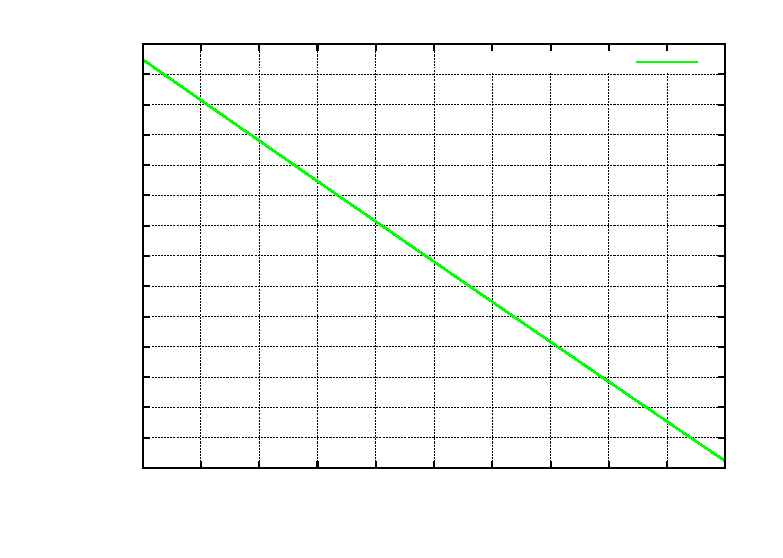
\includegraphics{../GNU/RLvhigh}}%
    \gplfronttext
  \end{picture}%
\endgroup
}
    \caption{Type 2 Messung}
    \label{fig:RLvhigh}
  \end{subfigure}
  \caption{Ausschnitt des theoretischen Spannungsverlauf von \(0\Omega\) bis \(10\Omega\)}
\end{figure}


\subsection{Widerstandsmessung mit den 470 kOhm Widerst\"anden}
Die n\"achsten Abbildungen~\ref{fig:RH1mes} und \ref{fig:RH2mes} zeigen die gleichen Me"smethoden f\"ur die Messungen mit
 \(470k\Omega\) Pr\"azisionswiderst\"anden.
Weil \(470k\Omega\) sehr gro"s ist in Relation zu den Port Widerst\"anden \(22\Omega\) und \(19\Omega\), 
k\"onnen die Port-Widerst\"ande f\"ur die Berechnung des Widerstandswertes Rx vernachl\"assigt werden.

F\"ur beide Me"smethoden mit den \(470k\Omega\) Widerst\"anden wird nur eine Spannung gemessen, weil der Strom
so niedrig ist, da"s keine Spannungsdifferenz an den internen Port Widerst\"anden gemessen werden kann (wie zu erwarten).
Der theoretische Spannungs-Verlauf wird in Abbildung~\ref{fig:RHv} gezeigt, wobei die Widerstandswerte wieder in
logarithmischer Skalierung gezeigt werden.
Der theoretische Verlauf in diesem Diagramm endet bei \(100M\Omega\), aber das Ergebnis des Testers wird auf
 \(60M\Omega\) begrenzt, anderenfalls nimmt der Tester an, da"s kein Widerstand angeschlossen ist.

\begin{figure}[H]
\centering

\includegraphics[]{../FIG/ResistormessH1.eps}
\caption{Messung Type 3 mit \(470k\Omega\) }
\label{fig:RH1mes}
\end{figure}

\begin{figure}[H]
 \centering
 
\includegraphics[]{../FIG/ResistormessH2.eps}
 \caption{Messung Type 4 mit \(470k\Omega\) }
\label{fig:RH2mes}
\end{figure}

\begin{figure}[H]
\centering
% GNUPLOT: LaTeX picture with Postscript
\begingroup
  \makeatletter
  \providecommand\color[2][]{%
    \GenericError{(gnuplot) \space\space\space\@spaces}{%
      Package color not loaded in conjunction with
      terminal option `colourtext'%
    }{See the gnuplot documentation for explanation.%
    }{Either use 'blacktext' in gnuplot or load the package
      color.sty in LaTeX.}%
    \renewcommand\color[2][]{}%
  }%
  \providecommand\includegraphics[2][]{%
    \GenericError{(gnuplot) \space\space\space\@spaces}{%
      Package graphicx or graphics not loaded%
    }{See the gnuplot documentation for explanation.%
    }{The gnuplot epslatex terminal needs graphicx.sty or graphics.sty.}%
    \renewcommand\includegraphics[2][]{}%
  }%
  \providecommand\rotatebox[2]{#2}%
  \@ifundefined{ifGPcolor}{%
    \newif\ifGPcolor
    \GPcolortrue
  }{}%
  \@ifundefined{ifGPblacktext}{%
    \newif\ifGPblacktext
    \GPblacktexttrue
  }{}%
  % define a \g@addto@macro without @ in the name:
  \let\gplgaddtomacro\g@addto@macro
  % define empty templates for all commands taking text:
  \gdef\gplbacktext{}%
  \gdef\gplfronttext{}%
  \makeatother
  \ifGPblacktext
    % no textcolor at all
    \def\colorrgb#1{}%
    \def\colorgray#1{}%
  \else
    % gray or color?
    \ifGPcolor
      \def\colorrgb#1{\color[rgb]{#1}}%
      \def\colorgray#1{\color[gray]{#1}}%
      \expandafter\def\csname LTw\endcsname{\color{white}}%
      \expandafter\def\csname LTb\endcsname{\color{black}}%
      \expandafter\def\csname LTa\endcsname{\color{black}}%
      \expandafter\def\csname LT0\endcsname{\color[rgb]{1,0,0}}%
      \expandafter\def\csname LT1\endcsname{\color[rgb]{0,1,0}}%
      \expandafter\def\csname LT2\endcsname{\color[rgb]{0,0,1}}%
      \expandafter\def\csname LT3\endcsname{\color[rgb]{1,0,1}}%
      \expandafter\def\csname LT4\endcsname{\color[rgb]{0,1,1}}%
      \expandafter\def\csname LT5\endcsname{\color[rgb]{1,1,0}}%
      \expandafter\def\csname LT6\endcsname{\color[rgb]{0,0,0}}%
      \expandafter\def\csname LT7\endcsname{\color[rgb]{1,0.3,0}}%
      \expandafter\def\csname LT8\endcsname{\color[rgb]{0.5,0.5,0.5}}%
    \else
      % gray
      \def\colorrgb#1{\color{black}}%
      \def\colorgray#1{\color[gray]{#1}}%
      \expandafter\def\csname LTw\endcsname{\color{white}}%
      \expandafter\def\csname LTb\endcsname{\color{black}}%
      \expandafter\def\csname LTa\endcsname{\color{black}}%
      \expandafter\def\csname LT0\endcsname{\color{black}}%
      \expandafter\def\csname LT1\endcsname{\color{black}}%
      \expandafter\def\csname LT2\endcsname{\color{black}}%
      \expandafter\def\csname LT3\endcsname{\color{black}}%
      \expandafter\def\csname LT4\endcsname{\color{black}}%
      \expandafter\def\csname LT5\endcsname{\color{black}}%
      \expandafter\def\csname LT6\endcsname{\color{black}}%
      \expandafter\def\csname LT7\endcsname{\color{black}}%
      \expandafter\def\csname LT8\endcsname{\color{black}}%
    \fi
  \fi
  \setlength{\unitlength}{0.0500bp}%
  \begin{picture}(7200.00,5040.00)%
    \gplgaddtomacro\gplbacktext{%
      \csname LTb\endcsname%
      \put(1078,704){\makebox(0,0)[r]{\strut{} 0}}%
      \csname LTb\endcsname%
      \put(1078,1518){\makebox(0,0)[r]{\strut{} 1000}}%
      \csname LTb\endcsname%
      \put(1078,2332){\makebox(0,0)[r]{\strut{} 2000}}%
      \csname LTb\endcsname%
      \put(1078,3147){\makebox(0,0)[r]{\strut{} 3000}}%
      \csname LTb\endcsname%
      \put(1078,3961){\makebox(0,0)[r]{\strut{} 4000}}%
      \csname LTb\endcsname%
      \put(1078,4775){\makebox(0,0)[r]{\strut{} 5000}}%
      \csname LTb\endcsname%
      \put(1210,484){\makebox(0,0){\strut{}10k}}%
      \csname LTb\endcsname%
      \put(2608,484){\makebox(0,0){\strut{}100k}}%
      \csname LTb\endcsname%
      \put(4007,484){\makebox(0,0){\strut{}1M}}%
      \csname LTb\endcsname%
      \put(5405,484){\makebox(0,0){\strut{}10M}}%
      \csname LTb\endcsname%
      \put(6803,484){\makebox(0,0){\strut{}100M}}%
      \put(176,2739){\rotatebox{-270}{\makebox(0,0){\strut{}voltage / mV}}}%
      \put(4006,154){\makebox(0,0){\strut{}resistor Rx / Ohm}}%
      \put(4006,4665){\makebox(0,0){\strut{}}}%
    }%
    \gplgaddtomacro\gplfronttext{%
      \csname LTb\endcsname%
      \put(5948,2874){\makebox(0,0)[r]{\strut{}PC2 type 3}}%
      \csname LTb\endcsname%
      \put(5948,2654){\makebox(0,0)[r]{\strut{}PC0, type 4}}%
    }%
    \gplbacktext
    \put(0,0){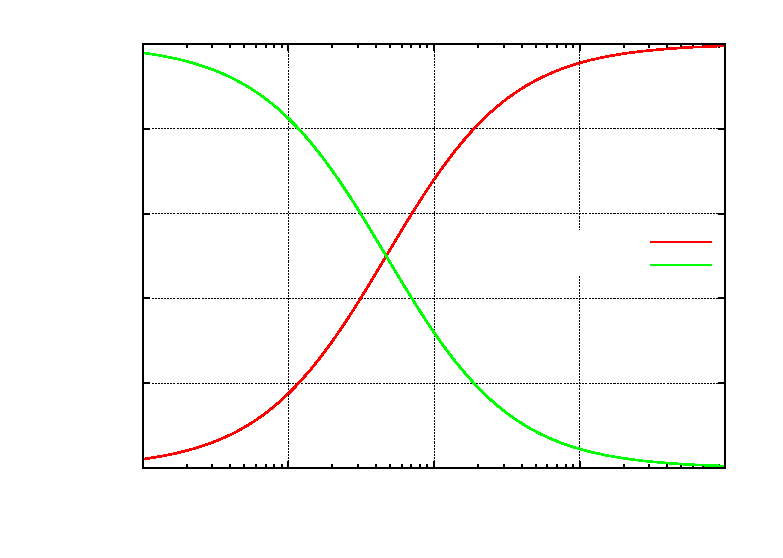
\includegraphics{../GNU/RHv}}%
    \gplfronttext
  \end{picture}%
\endgroup

\caption{Spannungen von Type 3 und Type 4 Messungen mit \(470k\Omega\) }
\label{fig:RHv}
\end{figure}

\subsection{Ergebnisse der Widerstands-Messung}
Abbildung~\ref{fig:mega8res} zeigt den relativen Fehler der Widerstandmessung mit einem ATmega8
Mikrocontroller. Mega8 sind die Ergebnisse ohne AUTOSCALE\_ADC Option,
Mega8as sind die Ergebnisse mit der Option AUTOSCALE\_ADC und
Mega8orig sind die gleichen Messungen mit der original Software von Markus F. ohne meine Verbesserungen.
Abbildung~\ref{fig:mega168res} zeigt die gleichen Messungen mit einem ATmega168 Mikrocontroller.
Mega168 sind die Ergebnisse ohne die AUTOSCALE\_ADC Option, Mega168as die mit der
 AUTOSCALE\_ADC Option.

Mit dem ATmega168 Mikrocontroller scheint es m\"oglich zu sein, Messungen von Widerst\"anden im
Bereich von \(20\Omega\) bis \(20M\Omega\) mit einem Me"sfehler von unter \(\pm1\%\) durchzuf\"uhren.
F\"ur Messungen unterhalb von \(100\Omega\) sollte man ber\"ucksichtigen, da"s jede Pr\"ufklemme mit Kabel ebenfalls
einen Widerstandwert hat.
Es ist besser, den Widerstand direkt mit den Anschlu"sklemmen zu verbinden.
Wenn das nicht m\"oglich ist, sollte man der Widerstandswert der kurzgeschlossenen Pr\"ufklemmen vom Me"sergebnis abziehen.
Zum Beispiel, wenn der Widerstand einen aufgedruckten Wert von \(30\Omega\) hat, der Tester zeigt
einen Wert von \(30,6\Omega\) an
und die beiden kurzgeschlossenen Pr\"ufklemmen haben einen Wert von \(0,5\Omega\), dann wird der Widerstand vom
Tester mit \(30,1\Omega\) gemessen.
Unterhalb von einem Widerstandswert von \(10\Omega\) macht ein Aufl\"osungs-Schritt von \(0,1\Omega\) schon einen Fehler von 1\%!

\begin{figure}[H]
\centering
% GNUPLOT: LaTeX picture with Postscript
\begingroup
  \makeatletter
  \providecommand\color[2][]{%
    \GenericError{(gnuplot) \space\space\space\@spaces}{%
      Package color not loaded in conjunction with
      terminal option `colourtext'%
    }{See the gnuplot documentation for explanation.%
    }{Either use 'blacktext' in gnuplot or load the package
      color.sty in LaTeX.}%
    \renewcommand\color[2][]{}%
  }%
  \providecommand\includegraphics[2][]{%
    \GenericError{(gnuplot) \space\space\space\@spaces}{%
      Package graphicx or graphics not loaded%
    }{See the gnuplot documentation for explanation.%
    }{The gnuplot epslatex terminal needs graphicx.sty or graphics.sty.}%
    \renewcommand\includegraphics[2][]{}%
  }%
  \providecommand\rotatebox[2]{#2}%
  \@ifundefined{ifGPcolor}{%
    \newif\ifGPcolor
    \GPcolortrue
  }{}%
  \@ifundefined{ifGPblacktext}{%
    \newif\ifGPblacktext
    \GPblacktexttrue
  }{}%
  % define a \g@addto@macro without @ in the name:
  \let\gplgaddtomacro\g@addto@macro
  % define empty templates for all commands taking text:
  \gdef\gplbacktext{}%
  \gdef\gplfronttext{}%
  \makeatother
  \ifGPblacktext
    % no textcolor at all
    \def\colorrgb#1{}%
    \def\colorgray#1{}%
  \else
    % gray or color?
    \ifGPcolor
      \def\colorrgb#1{\color[rgb]{#1}}%
      \def\colorgray#1{\color[gray]{#1}}%
      \expandafter\def\csname LTw\endcsname{\color{white}}%
      \expandafter\def\csname LTb\endcsname{\color{black}}%
      \expandafter\def\csname LTa\endcsname{\color{black}}%
      \expandafter\def\csname LT0\endcsname{\color[rgb]{1,0,0}}%
      \expandafter\def\csname LT1\endcsname{\color[rgb]{0,1,0}}%
      \expandafter\def\csname LT2\endcsname{\color[rgb]{0,0,1}}%
      \expandafter\def\csname LT3\endcsname{\color[rgb]{1,0,1}}%
      \expandafter\def\csname LT4\endcsname{\color[rgb]{0,1,1}}%
      \expandafter\def\csname LT5\endcsname{\color[rgb]{1,1,0}}%
      \expandafter\def\csname LT6\endcsname{\color[rgb]{0,0,0}}%
      \expandafter\def\csname LT7\endcsname{\color[rgb]{1,0.3,0}}%
      \expandafter\def\csname LT8\endcsname{\color[rgb]{0.5,0.5,0.5}}%
    \else
      % gray
      \def\colorrgb#1{\color{black}}%
      \def\colorgray#1{\color[gray]{#1}}%
      \expandafter\def\csname LTw\endcsname{\color{white}}%
      \expandafter\def\csname LTb\endcsname{\color{black}}%
      \expandafter\def\csname LTa\endcsname{\color{black}}%
      \expandafter\def\csname LT0\endcsname{\color{black}}%
      \expandafter\def\csname LT1\endcsname{\color{black}}%
      \expandafter\def\csname LT2\endcsname{\color{black}}%
      \expandafter\def\csname LT3\endcsname{\color{black}}%
      \expandafter\def\csname LT4\endcsname{\color{black}}%
      \expandafter\def\csname LT5\endcsname{\color{black}}%
      \expandafter\def\csname LT6\endcsname{\color{black}}%
      \expandafter\def\csname LT7\endcsname{\color{black}}%
      \expandafter\def\csname LT8\endcsname{\color{black}}%
    \fi
  \fi
  \setlength{\unitlength}{0.0500bp}%
  \begin{picture}(7200.00,5040.00)%
    \gplgaddtomacro\gplbacktext{%
      \csname LTb\endcsname%
      \put(682,704){\makebox(0,0)[r]{\strut{}-5}}%
      \csname LTb\endcsname%
      \put(682,1111){\makebox(0,0)[r]{\strut{}-4}}%
      \csname LTb\endcsname%
      \put(682,1518){\makebox(0,0)[r]{\strut{}-3}}%
      \csname LTb\endcsname%
      \put(682,1925){\makebox(0,0)[r]{\strut{}-2}}%
      \csname LTb\endcsname%
      \put(682,2332){\makebox(0,0)[r]{\strut{}-1}}%
      \csname LTb\endcsname%
      \put(682,2740){\makebox(0,0)[r]{\strut{} 0}}%
      \csname LTb\endcsname%
      \put(682,3147){\makebox(0,0)[r]{\strut{} 1}}%
      \csname LTb\endcsname%
      \put(682,3554){\makebox(0,0)[r]{\strut{} 2}}%
      \csname LTb\endcsname%
      \put(682,3961){\makebox(0,0)[r]{\strut{} 3}}%
      \csname LTb\endcsname%
      \put(682,4368){\makebox(0,0)[r]{\strut{} 4}}%
      \csname LTb\endcsname%
      \put(682,4775){\makebox(0,0)[r]{\strut{} 5}}%
      \csname LTb\endcsname%
      \put(814,484){\makebox(0,0){\strut{}1 }}%
      \csname LTb\endcsname%
      \put(1563,484){\makebox(0,0){\strut{}10 }}%
      \csname LTb\endcsname%
      \put(2311,484){\makebox(0,0){\strut{}100 }}%
      \csname LTb\endcsname%
      \put(3060,484){\makebox(0,0){\strut{}1k}}%
      \csname LTb\endcsname%
      \put(3809,484){\makebox(0,0){\strut{}10k}}%
      \csname LTb\endcsname%
      \put(4557,484){\makebox(0,0){\strut{}100k}}%
      \csname LTb\endcsname%
      \put(5306,484){\makebox(0,0){\strut{}1M}}%
      \csname LTb\endcsname%
      \put(6054,484){\makebox(0,0){\strut{}10M}}%
      \csname LTb\endcsname%
      \put(6803,484){\makebox(0,0){\strut{}100M}}%
      \put(176,2739){\rotatebox{-270}{\makebox(0,0){\strut{}Error / Percent}}}%
      \put(3808,154){\makebox(0,0){\strut{}Resistor value / Ohm}}%
    }%
    \gplgaddtomacro\gplfronttext{%
      \csname LTb\endcsname%
      \put(5753,4602){\makebox(0,0)[r]{\strut{}Mega8}}%
      \csname LTb\endcsname%
      \put(5753,4382){\makebox(0,0)[r]{\strut{}Mega8as}}%
      \csname LTb\endcsname%
      \put(5753,4162){\makebox(0,0)[r]{\strut{}Mega8orig}}%
    }%
    \gplbacktext
    \put(0,0){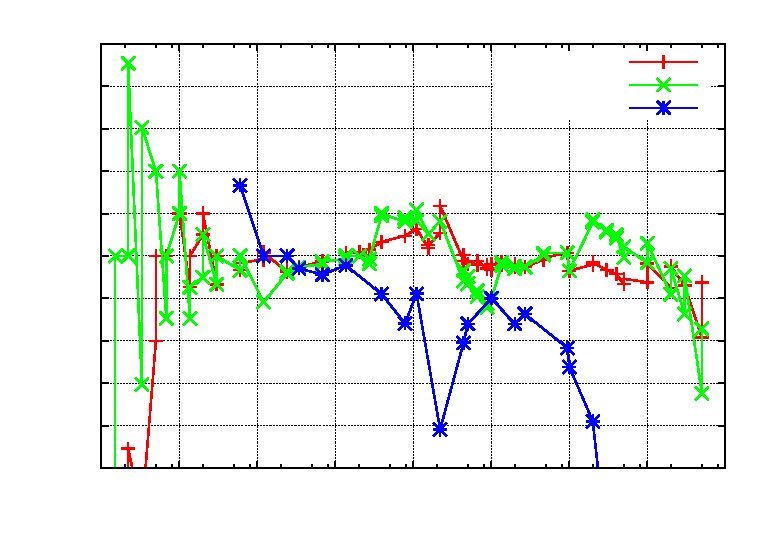
\includegraphics{../GNU/Mega8res}}%
    \gplfronttext
  \end{picture}%
\endgroup

\caption{Relativer Fehler in \% f\"ur Widerstands-Messungen mit ATmega8 }
\label{fig:mega8res}
\end{figure}

\begin{figure}[H]
\centering
% GNUPLOT: LaTeX picture with Postscript
\begingroup
  \makeatletter
  \providecommand\color[2][]{%
    \GenericError{(gnuplot) \space\space\space\@spaces}{%
      Package color not loaded in conjunction with
      terminal option `colourtext'%
    }{See the gnuplot documentation for explanation.%
    }{Either use 'blacktext' in gnuplot or load the package
      color.sty in LaTeX.}%
    \renewcommand\color[2][]{}%
  }%
  \providecommand\includegraphics[2][]{%
    \GenericError{(gnuplot) \space\space\space\@spaces}{%
      Package graphicx or graphics not loaded%
    }{See the gnuplot documentation for explanation.%
    }{The gnuplot epslatex terminal needs graphicx.sty or graphics.sty.}%
    \renewcommand\includegraphics[2][]{}%
  }%
  \providecommand\rotatebox[2]{#2}%
  \@ifundefined{ifGPcolor}{%
    \newif\ifGPcolor
    \GPcolortrue
  }{}%
  \@ifundefined{ifGPblacktext}{%
    \newif\ifGPblacktext
    \GPblacktexttrue
  }{}%
  % define a \g@addto@macro without @ in the name:
  \let\gplgaddtomacro\g@addto@macro
  % define empty templates for all commands taking text:
  \gdef\gplbacktext{}%
  \gdef\gplfronttext{}%
  \makeatother
  \ifGPblacktext
    % no textcolor at all
    \def\colorrgb#1{}%
    \def\colorgray#1{}%
  \else
    % gray or color?
    \ifGPcolor
      \def\colorrgb#1{\color[rgb]{#1}}%
      \def\colorgray#1{\color[gray]{#1}}%
      \expandafter\def\csname LTw\endcsname{\color{white}}%
      \expandafter\def\csname LTb\endcsname{\color{black}}%
      \expandafter\def\csname LTa\endcsname{\color{black}}%
      \expandafter\def\csname LT0\endcsname{\color[rgb]{1,0,0}}%
      \expandafter\def\csname LT1\endcsname{\color[rgb]{0,1,0}}%
      \expandafter\def\csname LT2\endcsname{\color[rgb]{0,0,1}}%
      \expandafter\def\csname LT3\endcsname{\color[rgb]{1,0,1}}%
      \expandafter\def\csname LT4\endcsname{\color[rgb]{0,1,1}}%
      \expandafter\def\csname LT5\endcsname{\color[rgb]{1,1,0}}%
      \expandafter\def\csname LT6\endcsname{\color[rgb]{0,0,0}}%
      \expandafter\def\csname LT7\endcsname{\color[rgb]{1,0.3,0}}%
      \expandafter\def\csname LT8\endcsname{\color[rgb]{0.5,0.5,0.5}}%
    \else
      % gray
      \def\colorrgb#1{\color{black}}%
      \def\colorgray#1{\color[gray]{#1}}%
      \expandafter\def\csname LTw\endcsname{\color{white}}%
      \expandafter\def\csname LTb\endcsname{\color{black}}%
      \expandafter\def\csname LTa\endcsname{\color{black}}%
      \expandafter\def\csname LT0\endcsname{\color{black}}%
      \expandafter\def\csname LT1\endcsname{\color{black}}%
      \expandafter\def\csname LT2\endcsname{\color{black}}%
      \expandafter\def\csname LT3\endcsname{\color{black}}%
      \expandafter\def\csname LT4\endcsname{\color{black}}%
      \expandafter\def\csname LT5\endcsname{\color{black}}%
      \expandafter\def\csname LT6\endcsname{\color{black}}%
      \expandafter\def\csname LT7\endcsname{\color{black}}%
      \expandafter\def\csname LT8\endcsname{\color{black}}%
    \fi
  \fi
  \setlength{\unitlength}{0.0500bp}%
  \begin{picture}(7200.00,5040.00)%
    \gplgaddtomacro\gplbacktext{%
      \csname LTb\endcsname%
      \put(682,704){\makebox(0,0)[r]{\strut{}-5}}%
      \csname LTb\endcsname%
      \put(682,1111){\makebox(0,0)[r]{\strut{}-4}}%
      \csname LTb\endcsname%
      \put(682,1518){\makebox(0,0)[r]{\strut{}-3}}%
      \csname LTb\endcsname%
      \put(682,1925){\makebox(0,0)[r]{\strut{}-2}}%
      \csname LTb\endcsname%
      \put(682,2332){\makebox(0,0)[r]{\strut{}-1}}%
      \csname LTb\endcsname%
      \put(682,2740){\makebox(0,0)[r]{\strut{} 0}}%
      \csname LTb\endcsname%
      \put(682,3147){\makebox(0,0)[r]{\strut{} 1}}%
      \csname LTb\endcsname%
      \put(682,3554){\makebox(0,0)[r]{\strut{} 2}}%
      \csname LTb\endcsname%
      \put(682,3961){\makebox(0,0)[r]{\strut{} 3}}%
      \csname LTb\endcsname%
      \put(682,4368){\makebox(0,0)[r]{\strut{} 4}}%
      \csname LTb\endcsname%
      \put(682,4775){\makebox(0,0)[r]{\strut{} 5}}%
      \csname LTb\endcsname%
      \put(814,484){\makebox(0,0){\strut{}1 }}%
      \csname LTb\endcsname%
      \put(1563,484){\makebox(0,0){\strut{}10 }}%
      \csname LTb\endcsname%
      \put(2311,484){\makebox(0,0){\strut{}100 }}%
      \csname LTb\endcsname%
      \put(3060,484){\makebox(0,0){\strut{}1k}}%
      \csname LTb\endcsname%
      \put(3809,484){\makebox(0,0){\strut{}10k}}%
      \csname LTb\endcsname%
      \put(4557,484){\makebox(0,0){\strut{}100k}}%
      \csname LTb\endcsname%
      \put(5306,484){\makebox(0,0){\strut{}1M}}%
      \csname LTb\endcsname%
      \put(6054,484){\makebox(0,0){\strut{}10M}}%
      \csname LTb\endcsname%
      \put(6803,484){\makebox(0,0){\strut{}100M}}%
      \put(176,2739){\rotatebox{-270}{\makebox(0,0){\strut{}Error / Percent}}}%
      \put(3808,154){\makebox(0,0){\strut{}Resistor value / Ohm}}%
    }%
    \gplgaddtomacro\gplfronttext{%
      \csname LTb\endcsname%
      \put(5753,4602){\makebox(0,0)[r]{\strut{}Mega168}}%
      \csname LTb\endcsname%
      \put(5753,4382){\makebox(0,0)[r]{\strut{}Mega168as}}%
    }%
    \gplbacktext
    \put(0,0){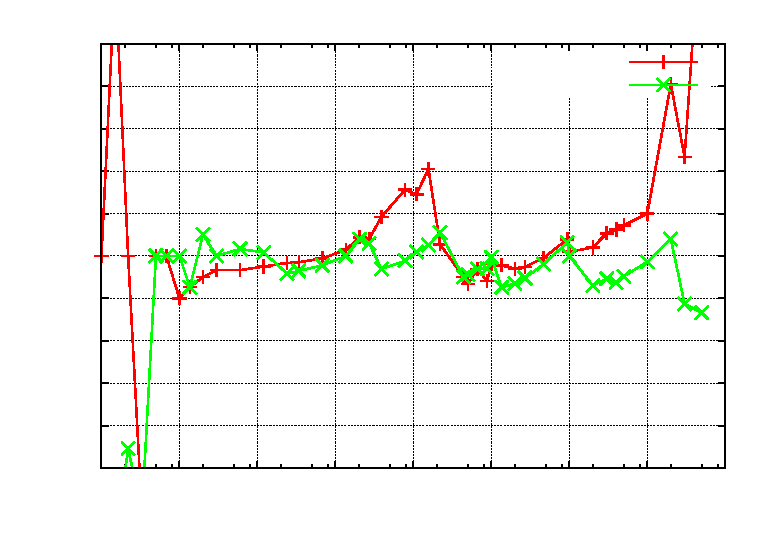
\includegraphics{../GNU/Mega168res}}%
    \gplfronttext
  \end{picture}%
\endgroup

\caption{Relativer Fehler in \% f\"ur Widerstand-Messungen mit ATmega168 }
\label{fig:mega168res}
\end{figure}
